\usepackage{listingsutf8}
\usepackage[utf8]{inputenc}
\usepackage[T1]{fontenc}
\usepackage{xcolor}
\usepackage{hyperref}
\usepackage{textpos}

\usetheme{CambridgeUS}
\setbeamerfont{frametitle}{size=\large}
\useinnertheme{circles}
\usefonttheme{professionalfonts}

\title{Git a look under the hood}
\subtitle{Build a deeper understanding of gits internals}
\author{Vincent Scherb}
\institute[IPI GmbH]{
\includegraphics[height=1cm]{images/ipi-logo.png}\\IPI GmbH}
\date{\today}

\AtBeginSection[]
{
    \begin{frame}<beamer>
        \frametitle{Table of Contents}
        \tableofcontents[currentsection]
    \end{frame}
}

\addtobeamertemplate{frametitle}{}{
    \begin{textblock*}{100mm}(.9\textwidth,-.65cm)
        
\includegraphics[height=.5cm]{images/ipi-logo.png}
    \end{textblock*}
}

\setbeamertemplate{navigation symbols}{}



% source: https://tex.stackexchange.com/questions/46953/unix-command-highlighting-latex/46994#46994
\lstdefinestyle{BashInputStyle}{
    language=bash,
    basicstyle=\small\ttfamily,
    numbers=left,
    numberstyle=\tiny,
    numbersep=3pt,
    frame=tb,
    columns=fullflexible,
    backgroundcolor=\color{yellow!20},
    linewidth=0.9\linewidth,
    xleftmargin=0.1\linewidth,
    breaklines=true
}

\begin{document}
    \frame{\titlepage}

    \section*{Table of Contents}
    \begin{frame}
        \frametitle{Table of Contents}
        \tableofcontents
    \end{frame}

    \section*{Introduction}
\begin{frame}
    \frametitle{Introduction}

\end{frame}



    \section{Contents of .git directory}
\subsection{.git directory folder structure}
\begin{frame}[fragile]
    \frametitle{.git root directory}
    \begin{figure}
        \begin{center}
            \ifnumequal{\aspectratio}{43}
            {
                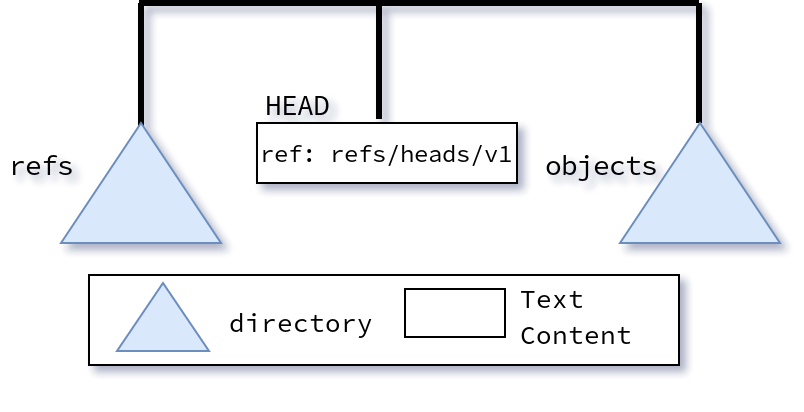
\includegraphics[width=0.75\textwidth,keepaspectratio]{./images/gitDirectory-Root.png}
            }
            {
                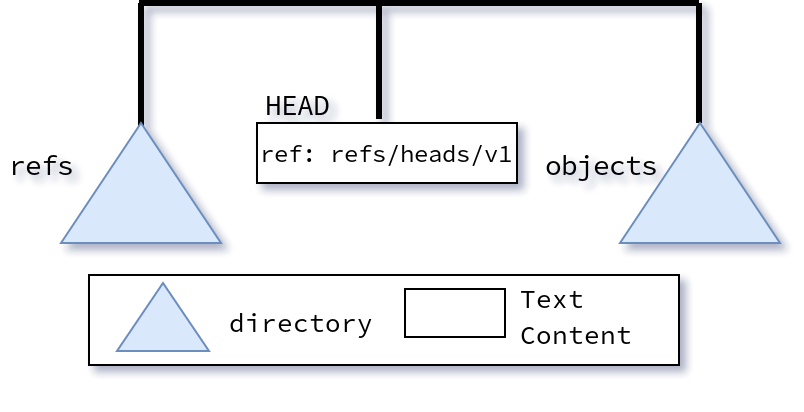
\includegraphics[height=0.75\textheight,keepaspectratio]{./images/gitDirectory-Root.png}
            }
            \caption{.git root directory}
        \end{center}
    \end{figure}
\end{frame}




    \begin{frame}[fragile]
    \frametitle{.git directory Refs}
    \begin{figure}
        \begin{center}
            \ifnumequal{\aspectratio}{43}
            {
                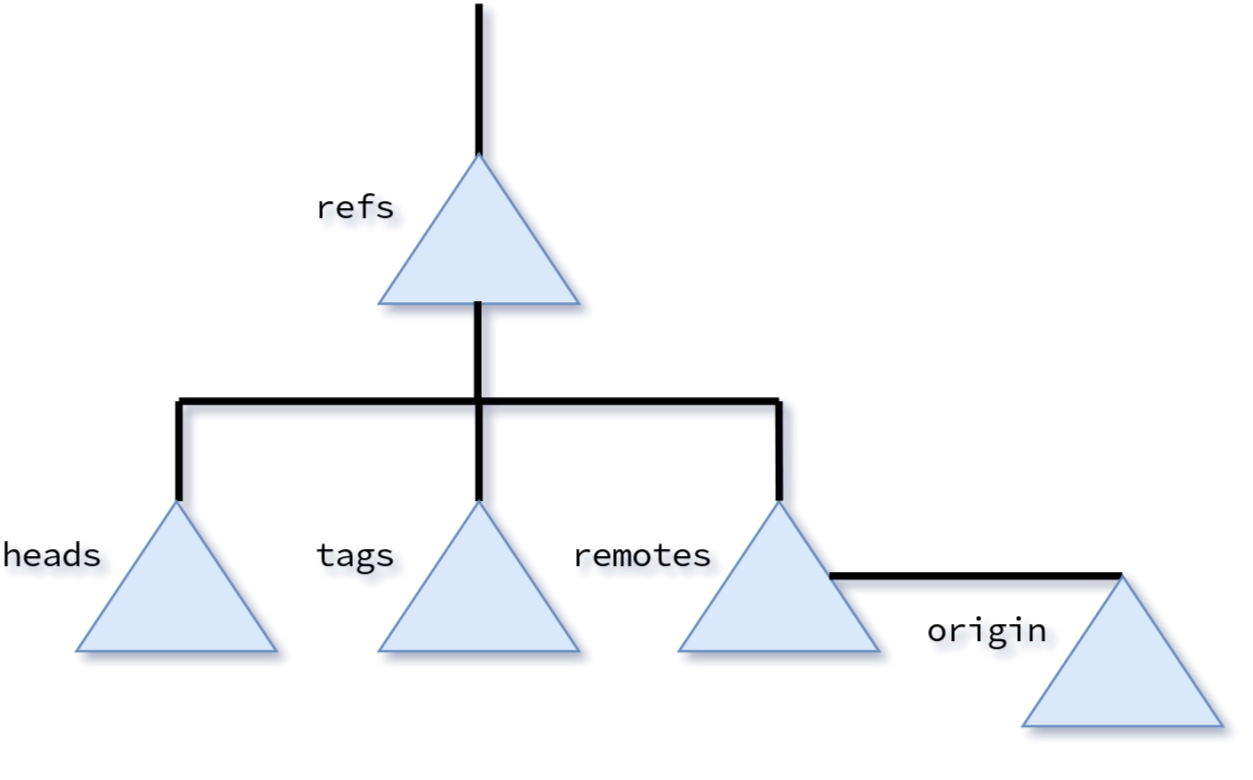
\includegraphics[height=0.75\textheight,keepaspectratio]{./images/gitDirectory-Refs.png}
            }
            {
                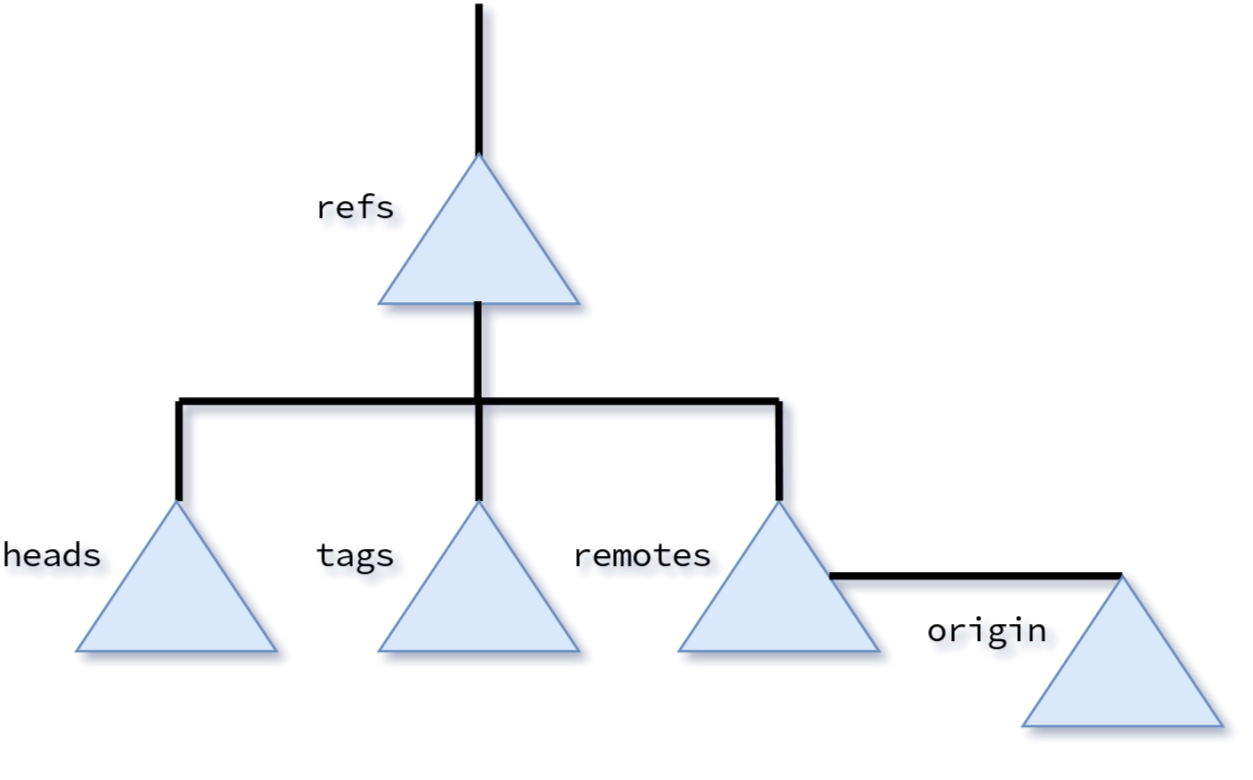
\includegraphics[height=0.75\textheight,width=0.8\textwidth]{./images/gitDirectory-Refs.png}
            }
            \caption{.git directory Refs}
        \end{center}
    \end{figure}
\end{frame}



    \begin{frame}[fragile,noframenumbering]
    \frametitle{.git directory Refs with content}
    \addtocounter{page}{-1}
    \begin{figure}
        \begin{center}
            \ifnumequal{\aspectratio}{43}
            {
                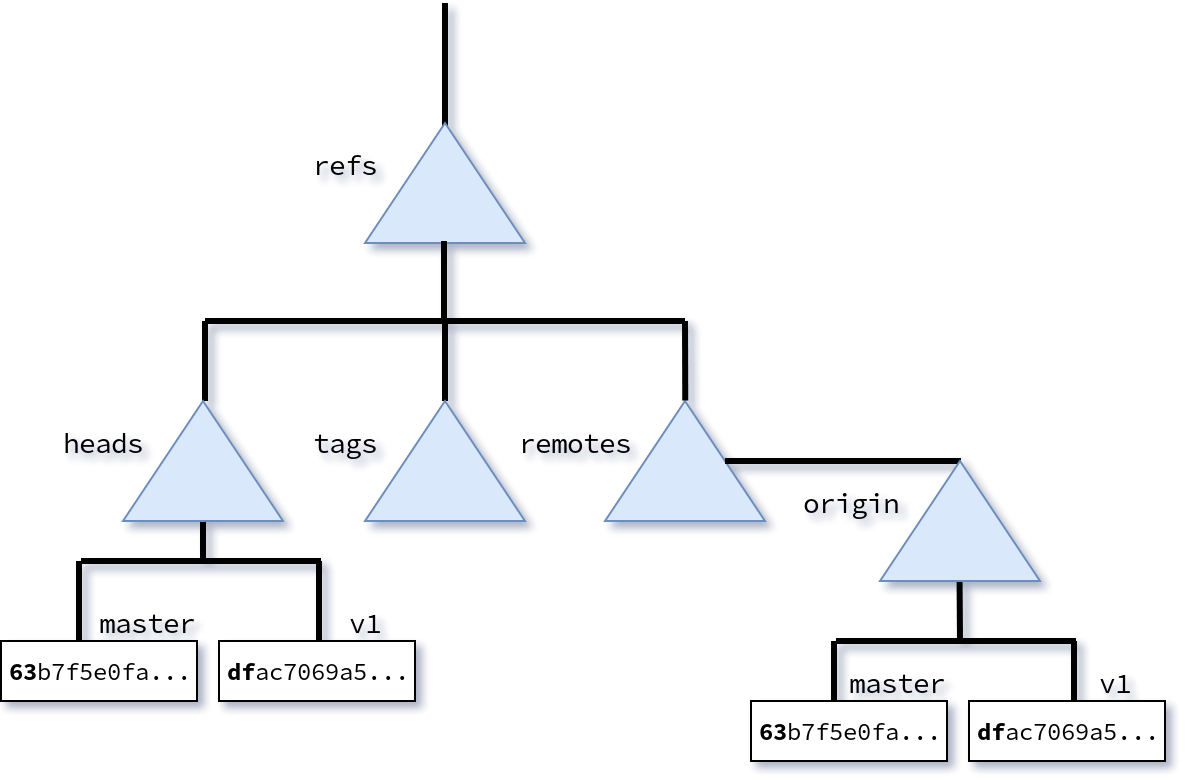
\includegraphics[height=0.75\textheight,keepaspectratio]{./images/gitDirectory-Refs_Content.png}
            }
            {
                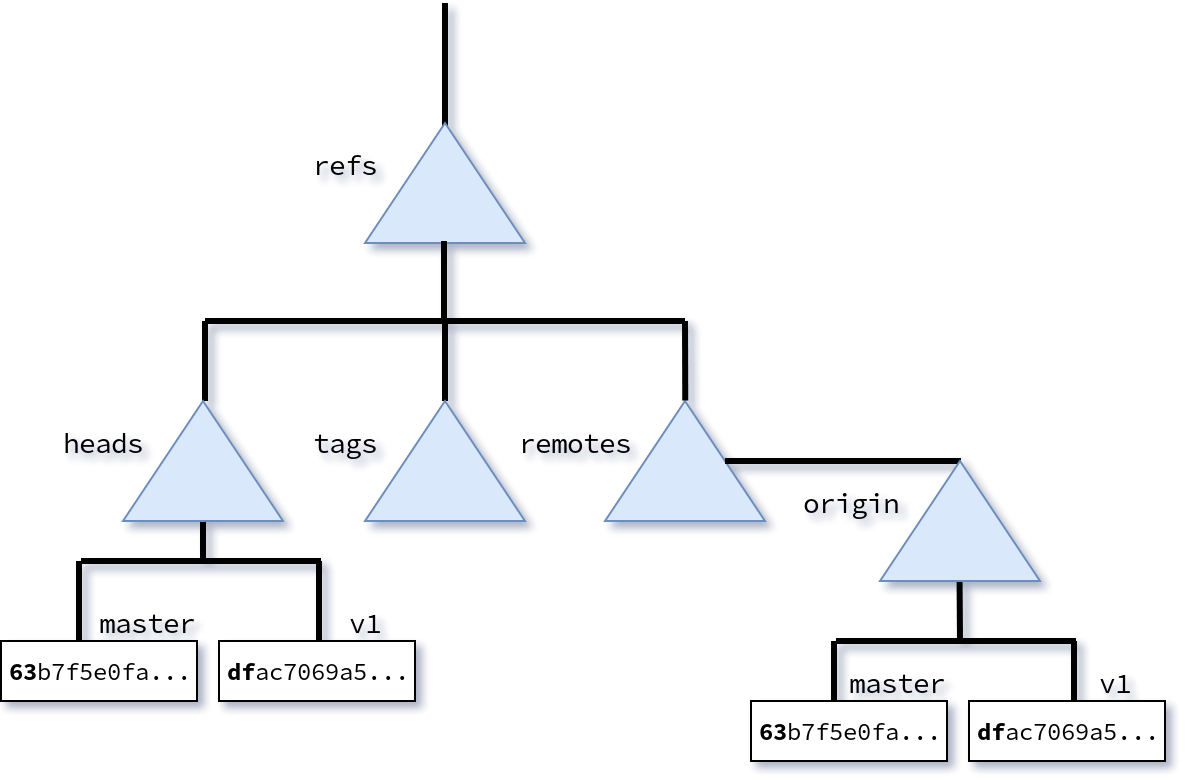
\includegraphics[height=0.75\textheight,width=0.8\textwidth]{./images/gitDirectory-Refs_Content.png}
            }
            \caption{.git directory Refs with content}
        \end{center}
    \end{figure}
\end{frame}



    \section{Contents of .git directory}
\begin{frame}[fragile]
    \frametitle{Exploring the .git directory}
    \begin{figure}
        \begin{center}
            \ifnumequal{\aspectratio}{43}
            {
                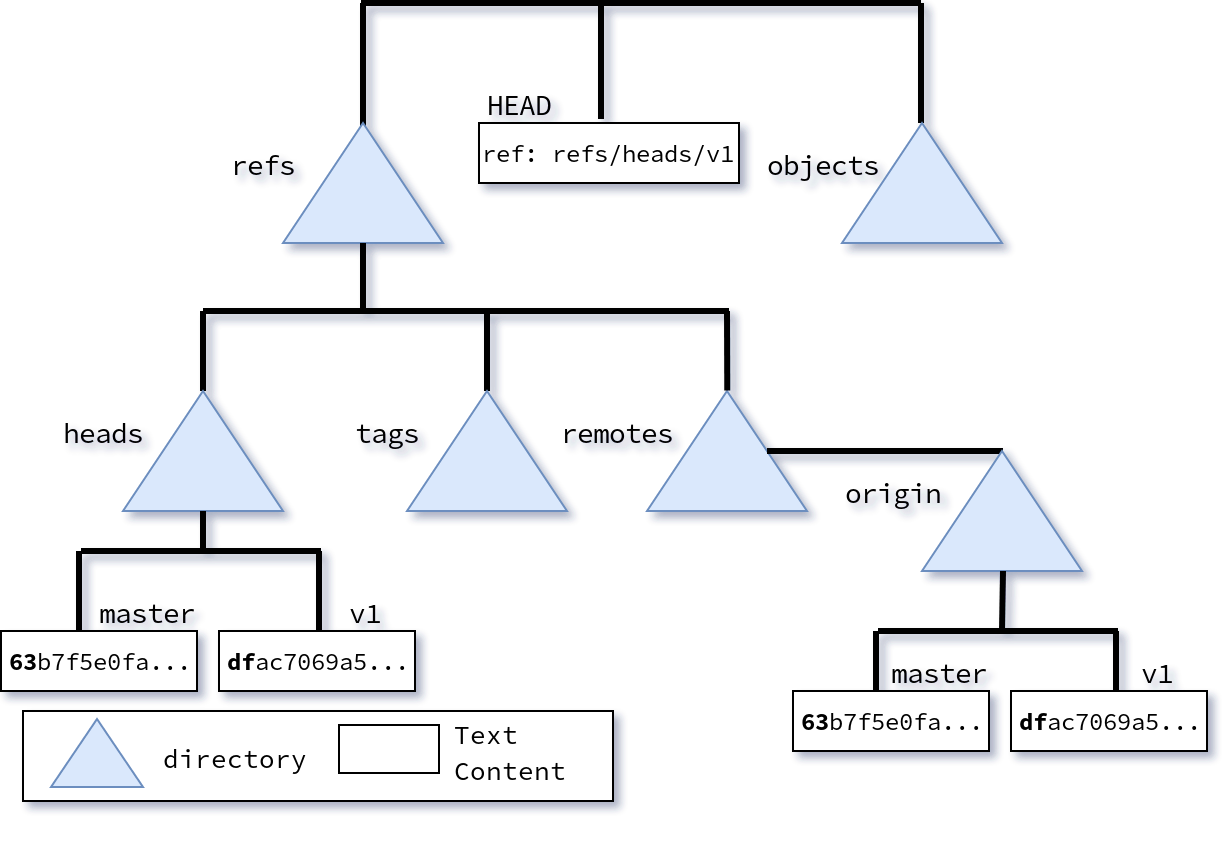
\includegraphics[height=0.75\textheight,keepaspectratio]{./images/gitDirectory.png}
            }
            {
                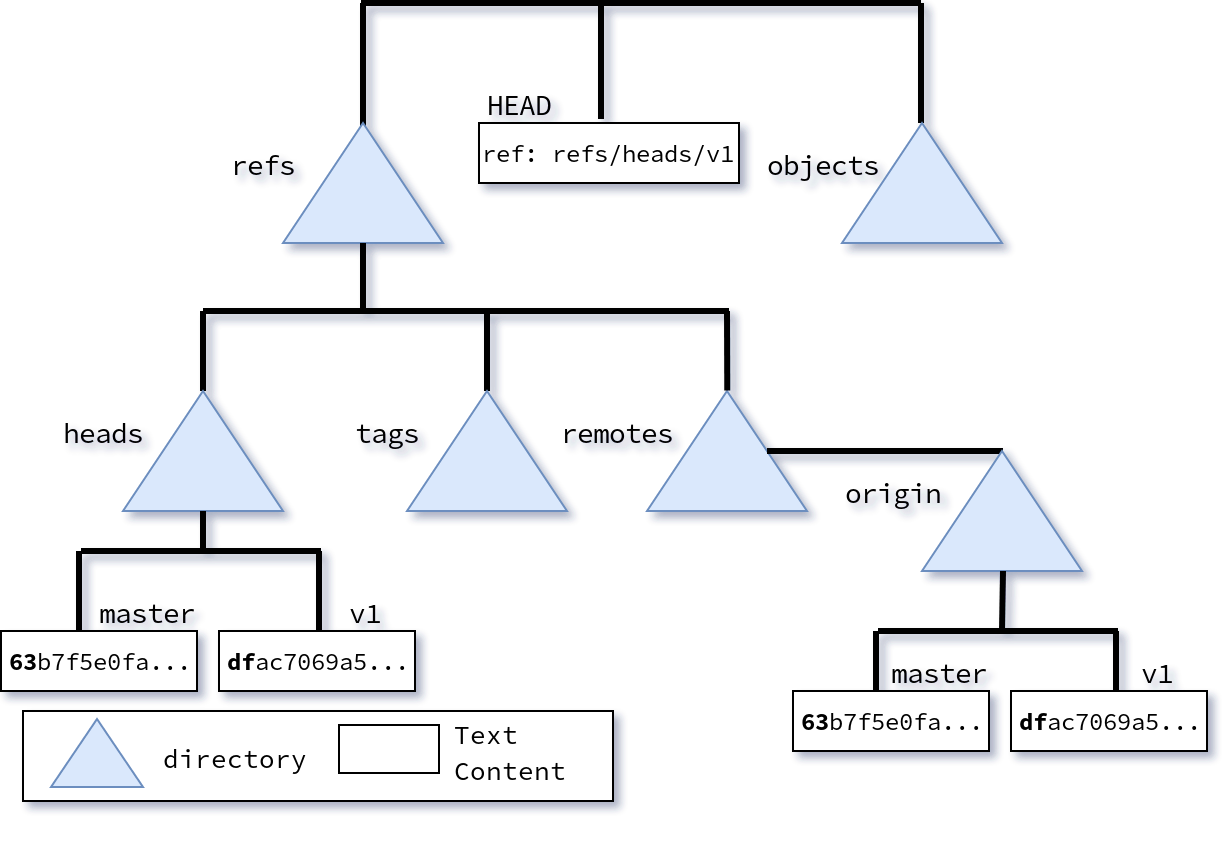
\includegraphics[height=0.75\textheight,width=0.8\textwidth]{./images/gitDirectory.png}
            }
            \caption{.git directory}
        \end{center}
    \end{figure}
\end{frame}



    \subsection{objects}
\begin{frame}[fragile]
    \frametitle{Exploring the objects directory}
    \lstset{
        language=bash,
        showstringspaces=true,
        frame=single,
        style=BashInputStyle
    }
    \begin{lstlisting}[caption={git log --raw -n1}, label={fig:lograw}]
commit d8c22f8205cab34e00e6a172febedd6d5f1a2ada (HEAD -> master)
Author: [...]
Date:   [...]

    Git directory Root added

:100644 100644 dbd87be bccdfbd M        README
:000000 100644 0000000 1b16bf9 A        images/gitDirectory-Root.png
:000000 100644 0000000 013543d A        slides/GitDirectoryRoot.tex
    \end{lstlisting}
\end{frame}

\begin{frame}[fragile]
    \frametitle{objects directory}
    \lstset{
        language=bash,
        showstringspaces=true,
        frame=single,
        style=BashInputStyle
    }
    \begin{lstlisting}[caption={[Tree]tree .git/objects example (shortened with comments)},label={fig:objectsdirectory}]
./.git/objects
|-- 87
|   |-- ccb1974b8bbcb39aa6c6bedc13a27bd4308142 tree
|-- bc
|   |-- cdfbd6314e19a21c367ba5ea9cbe65a1a0818e blob
|-- d2
|   |-- e82a9df8b4521fb6b25f22fb87ffe0e873413c staged blob
|-- d8
|   |-- c22f8205cab34e00e6a172febedd6d5f1a2ada commit
|-- info
|-- pack
    \end{lstlisting}
\end{frame}



    \section{Git areas}
\subsection{The stages of Git}
\begin{frame}[fragile]
    \frametitle{Different areas in git}
    \begin{figure}
        \begin{center}
            \ifnumequal{\aspectratio}{43}
            {
                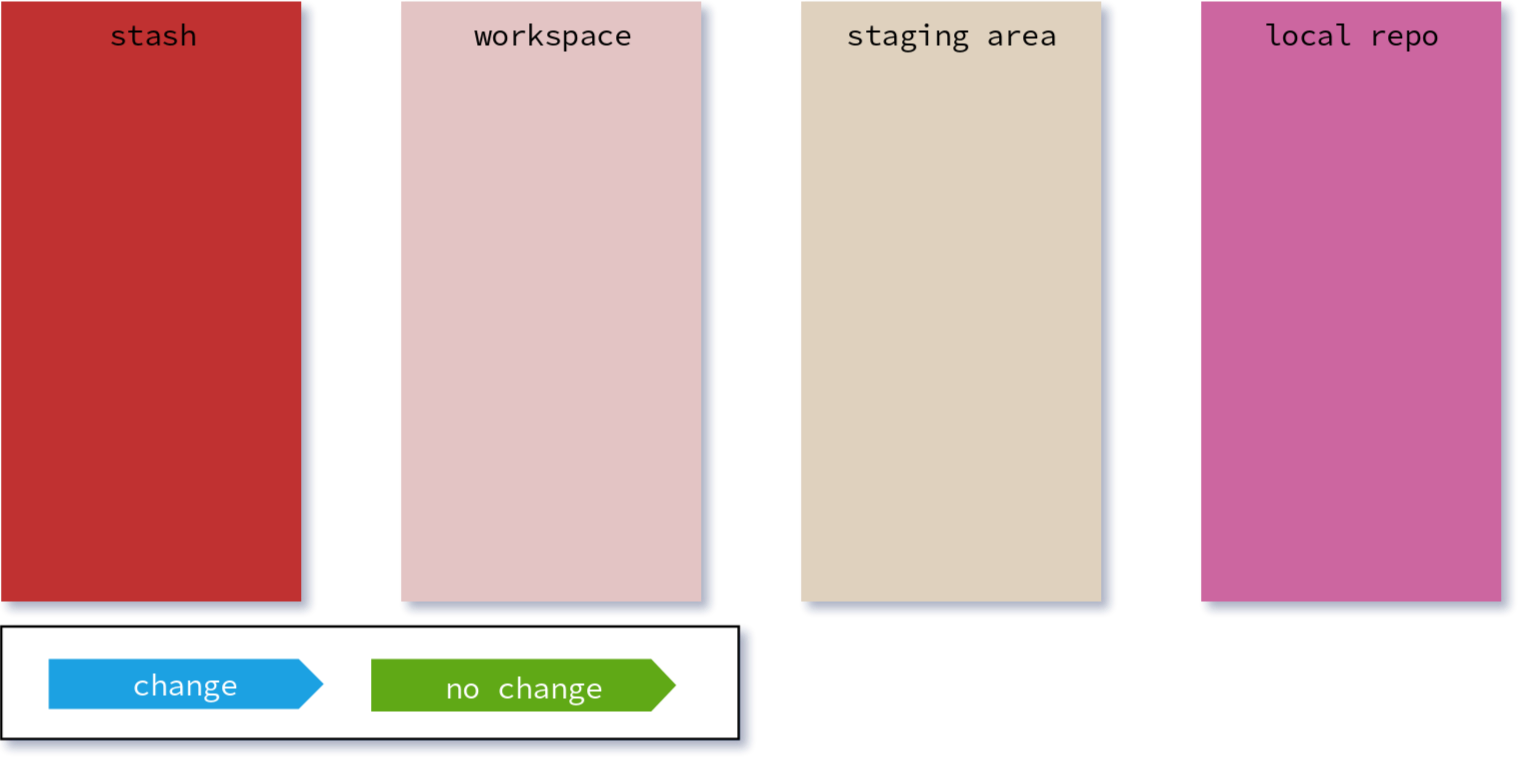
\includegraphics[width=1\textwidth,keepaspectratio]{./images/GitAreas.png}
            }
            {
                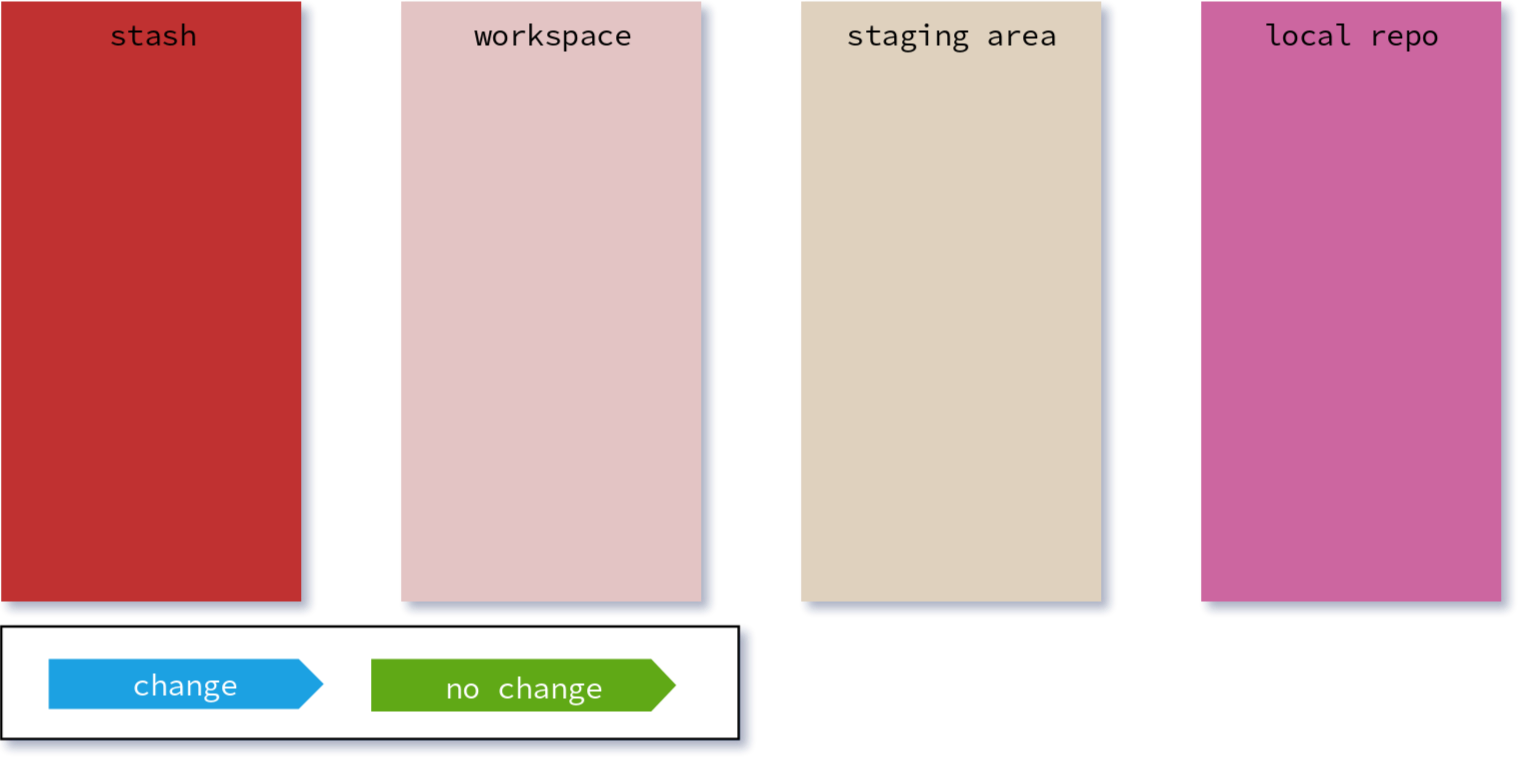
\includegraphics[height=0.75\textheight,keepaspectratio]{./images/GitAreas.png}
            }
            \caption{Areas in git}
        \end{center}
    \end{figure}
\end{frame}

\subsection*{Git workspace}
\begin{frame}[fragile]
    \frametitle{Git Workspace}
    \begin{figure}
        \begin{center}
            \ifnumequal{\aspectratio}{43}
            {
                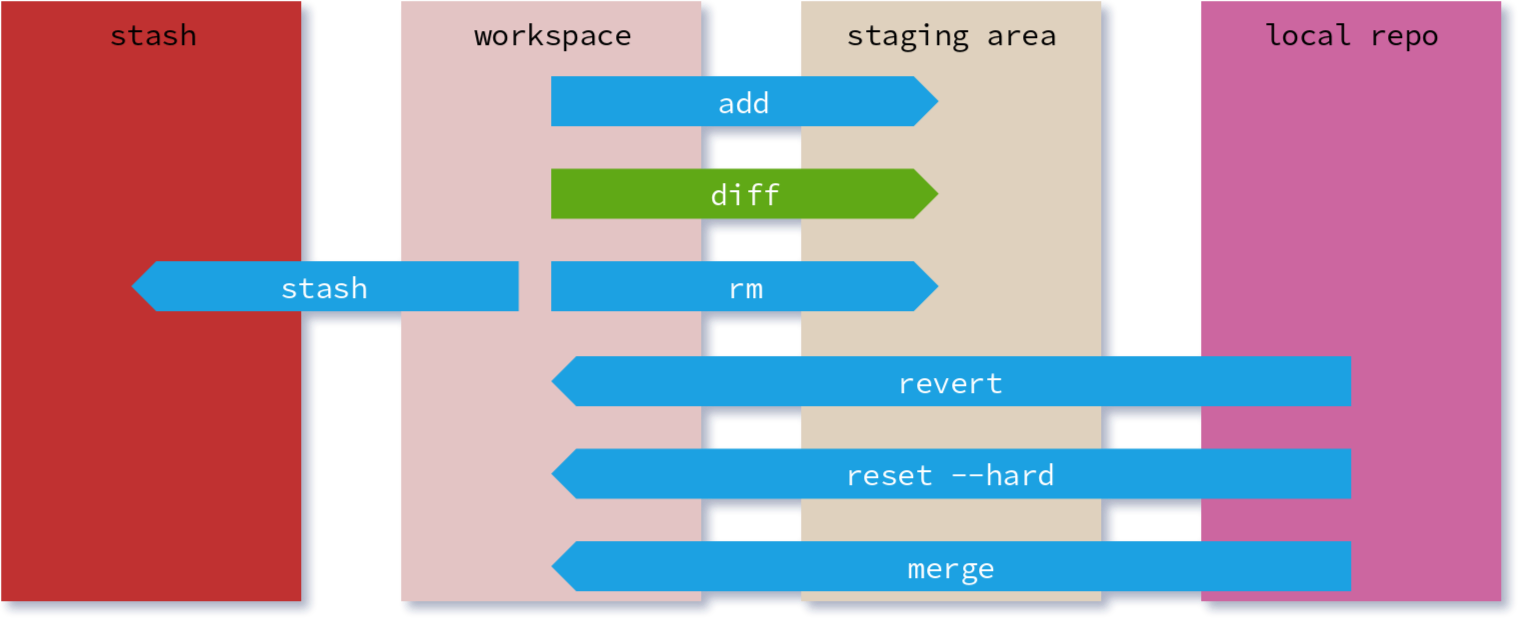
\includegraphics[width=1\textwidth,keepaspectratio]{./images/GitAreas-Workspace.png}
            }
            {
                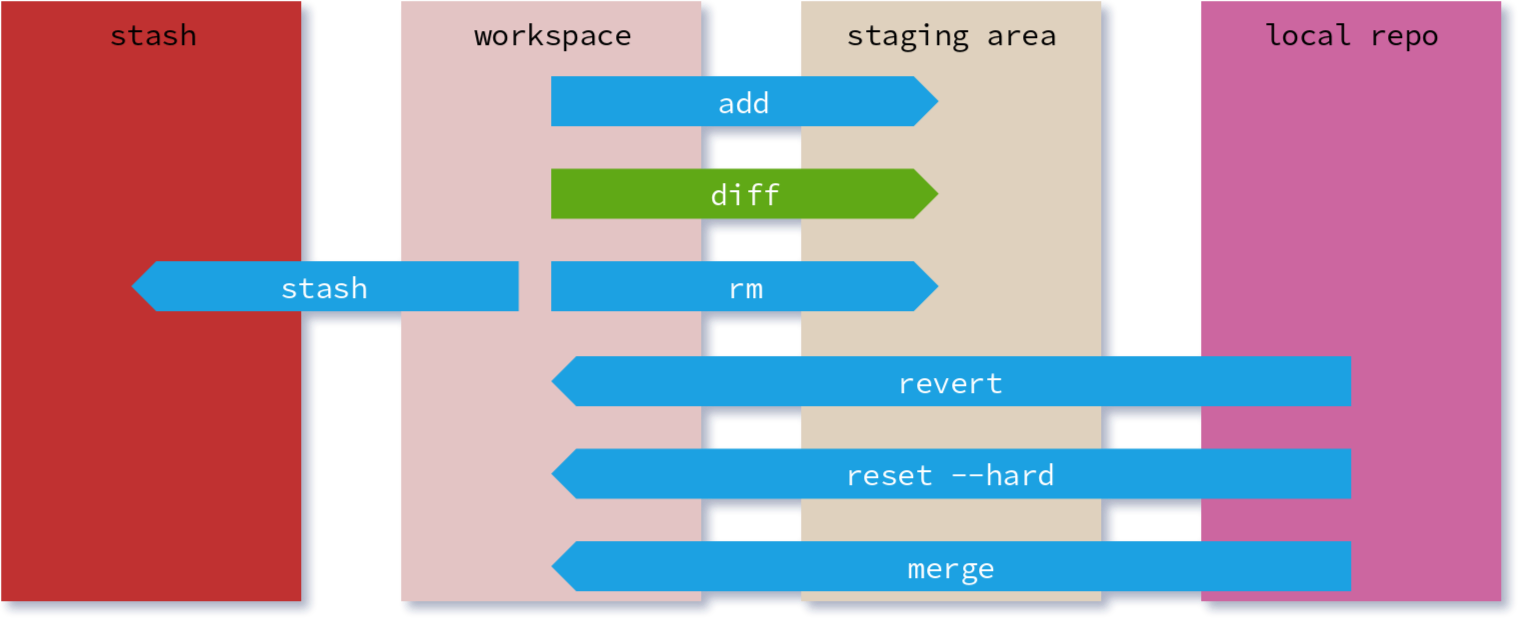
\includegraphics[height=0.75\textheight,keepaspectratio]{./images/GitAreas-Workspace.png}
            }
            \caption{Workspace area}
        \end{center}
    \end{figure}
\end{frame}

\subsection*{Git staging}
\begin{frame}[fragile]
    \frametitle{Git Staging}
    \begin{figure}
        \begin{center}
            \ifnumequal{\aspectratio}{43}
            {
                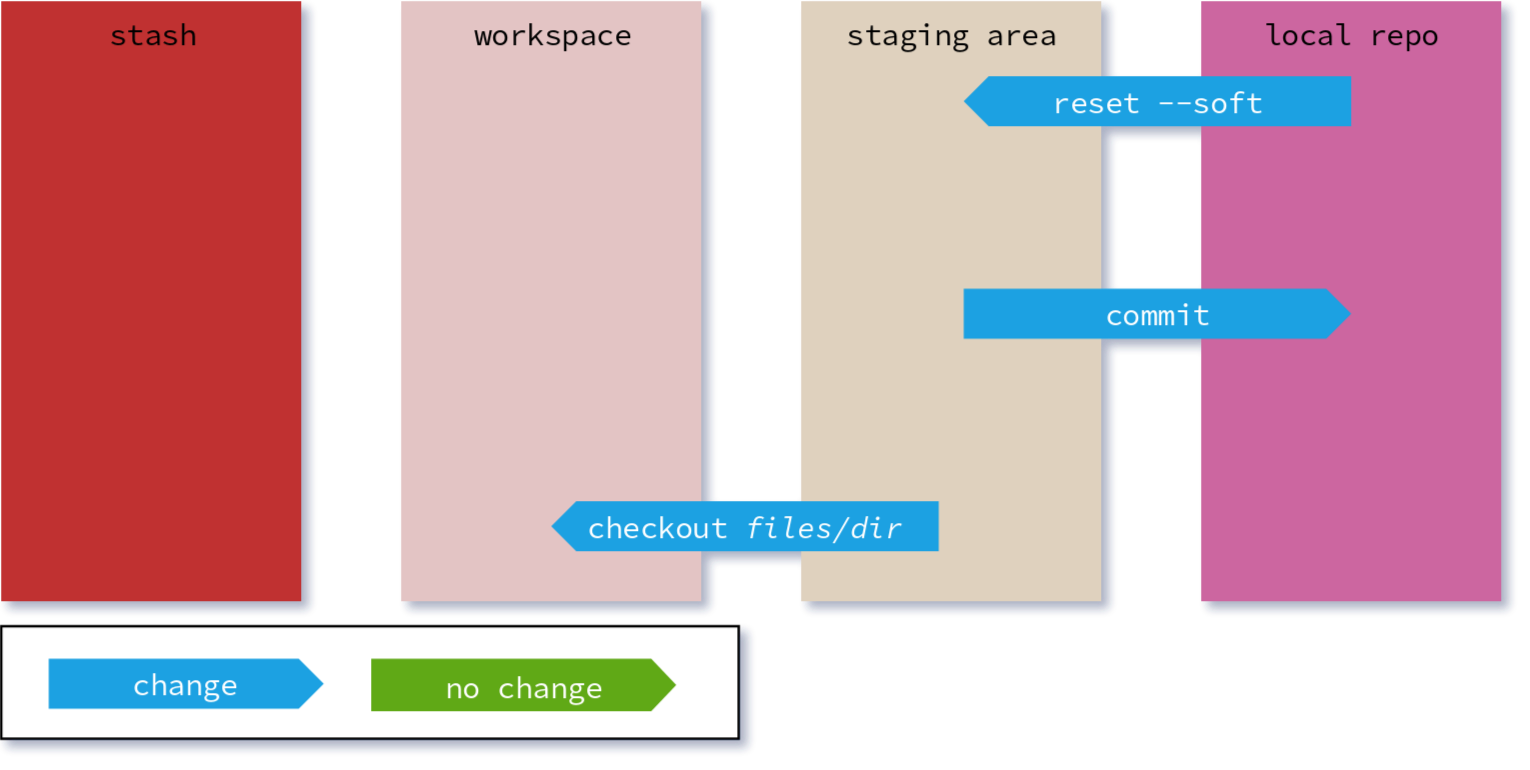
\includegraphics[width=1\textwidth,keepaspectratio]{./images/GitAreas-Staging.png}
            }
            {
                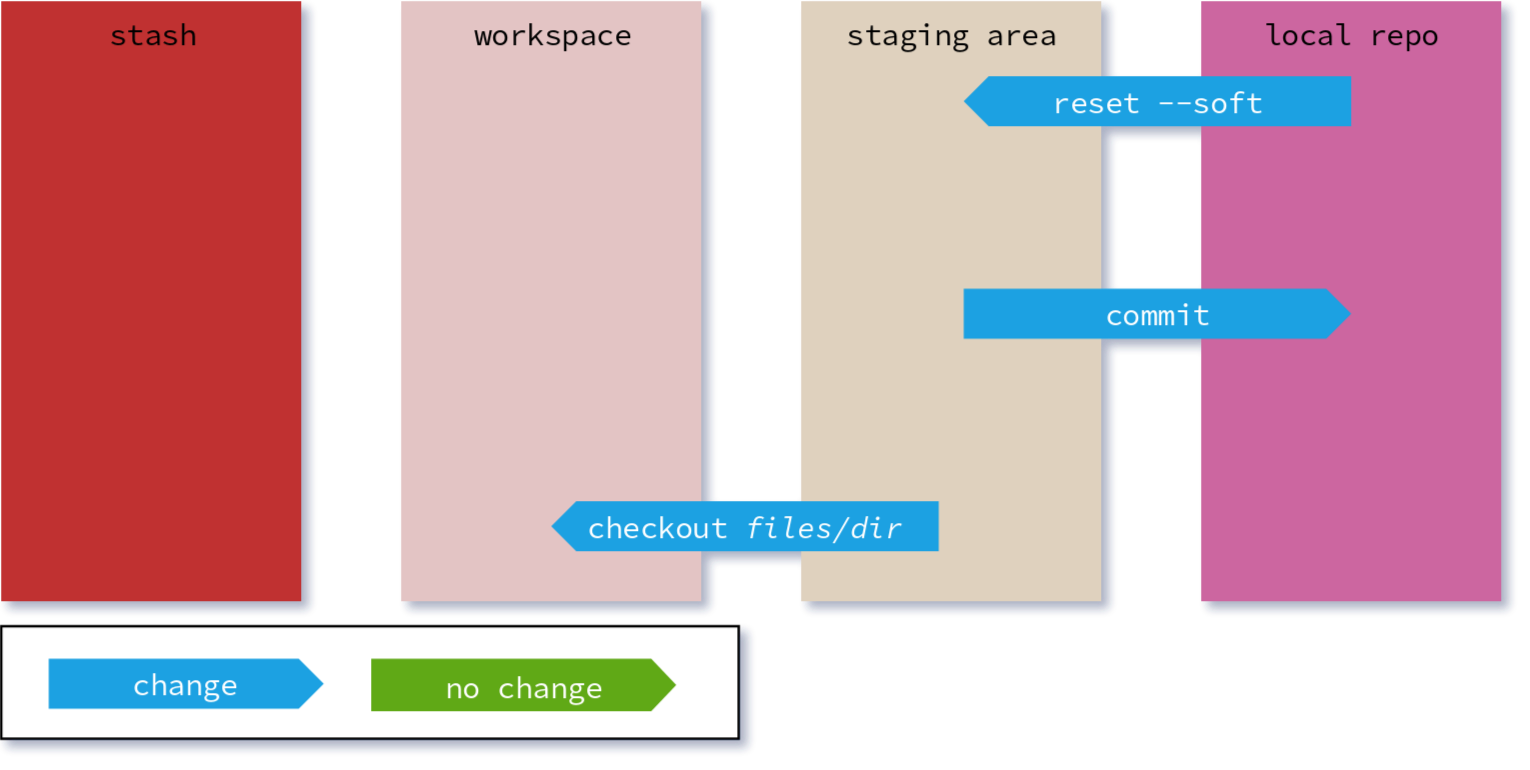
\includegraphics[height=0.75\textheight,keepaspectratio]{./images/GitAreas-Staging.png}
            }
            \caption{Staging area}
        \end{center}
    \end{figure}
\end{frame}

\subsection*{Git local repository}
\begin{frame}[fragile]
    \frametitle{Git local repository}
    \begin{figure}
        \begin{center}
            \ifnumequal{\aspectratio}{43}
            {
                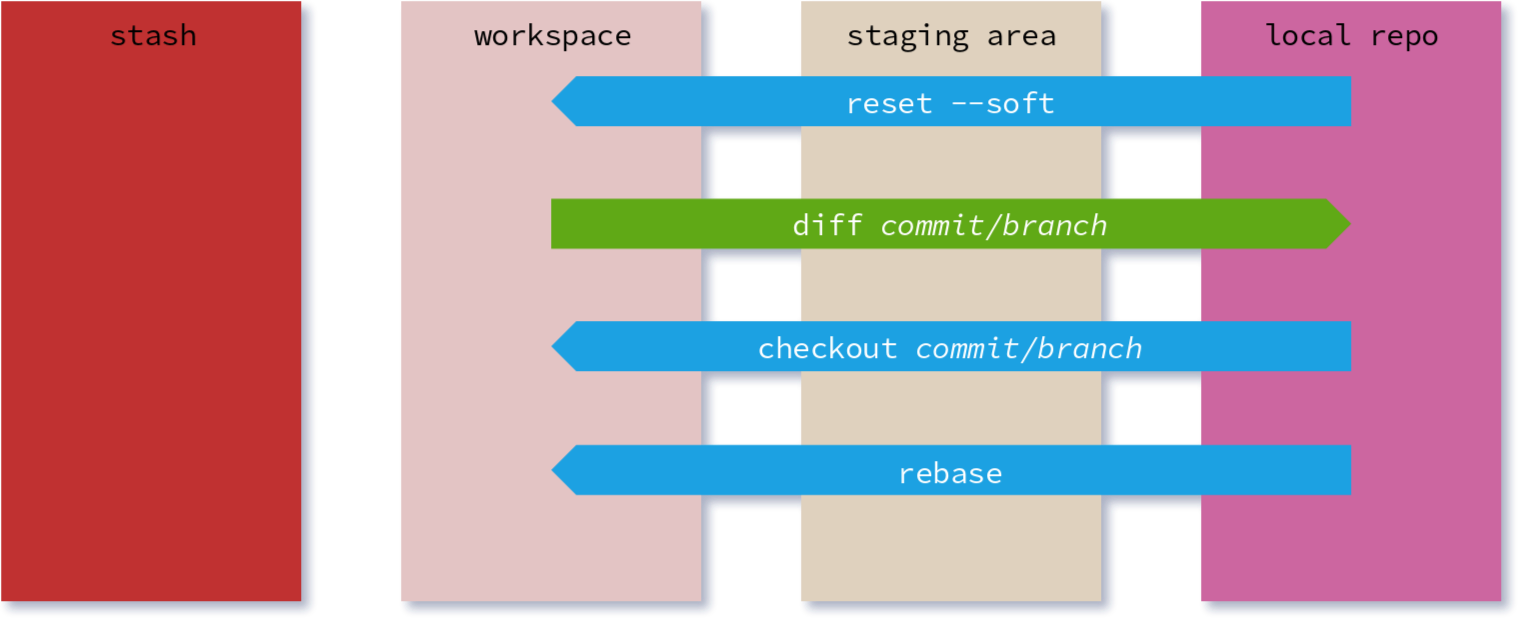
\includegraphics[width=1\textwidth,keepaspectratio]{./images/GitAreas-LocalRepo.png}
            }
            {
                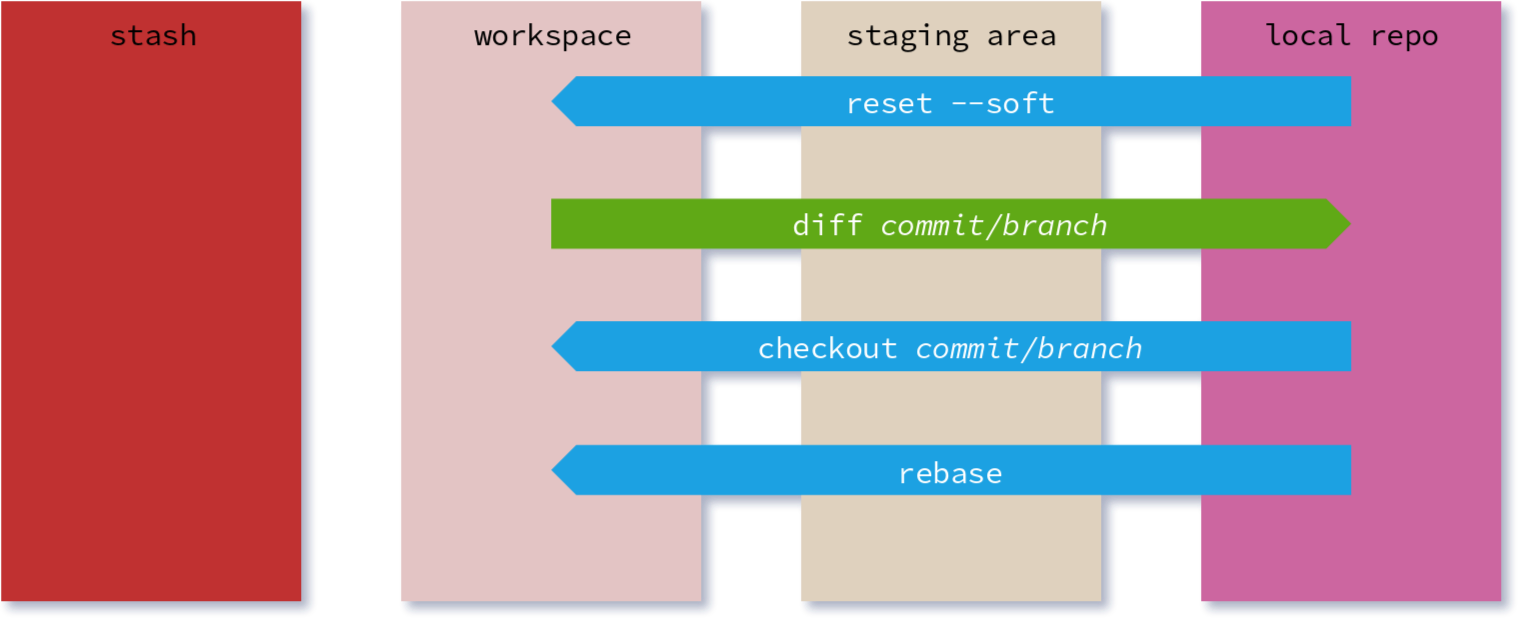
\includegraphics[height=0.75\textheight,keepaspectratio]{./images/GitAreas-LocalRepo.png}
            }
            \caption{Local repository area}
        \end{center}
    \end{figure}
\end{frame}



    \subsection{Recap}
\begin{frame}
    \frametitle{Recap Git areas}
    \begin{itemize}
        \item Three areas where you mainly work
            \begin{itemize}
                \item workspace
                \item staging also called index
                \item local repository
            \end{itemize}
        \item Most commands move changes between those areas
    \end{itemize}
\end{frame}



\end{document}

